







\documentclass{article}\usepackage[]{graphicx}\usepackage[]{color}
%% maxwidth is the original width if it is less than linewidth
%% otherwise use linewidth (to make sure the graphics do not exceed the margin)
\makeatletter
\def\maxwidth{ %
  \ifdim\Gin@nat@width>\linewidth
    \linewidth
  \else
    \Gin@nat@width
  \fi
}
\makeatother

\definecolor{fgcolor}{rgb}{0.345, 0.345, 0.345}
\newcommand{\hlnum}[1]{\textcolor[rgb]{0.686,0.059,0.569}{#1}}%
\newcommand{\hlstr}[1]{\textcolor[rgb]{0.192,0.494,0.8}{#1}}%
\newcommand{\hlcom}[1]{\textcolor[rgb]{0.678,0.584,0.686}{\textit{#1}}}%
\newcommand{\hlopt}[1]{\textcolor[rgb]{0,0,0}{#1}}%
\newcommand{\hlstd}[1]{\textcolor[rgb]{0.345,0.345,0.345}{#1}}%
\newcommand{\hlkwa}[1]{\textcolor[rgb]{0.161,0.373,0.58}{\textbf{#1}}}%
\newcommand{\hlkwb}[1]{\textcolor[rgb]{0.69,0.353,0.396}{#1}}%
\newcommand{\hlkwc}[1]{\textcolor[rgb]{0.333,0.667,0.333}{#1}}%
\newcommand{\hlkwd}[1]{\textcolor[rgb]{0.737,0.353,0.396}{\textbf{#1}}}%

\usepackage{framed}
\makeatletter
\newenvironment{kframe}{%
 \def\at@end@of@kframe{}%
 \ifinner\ifhmode%
  \def\at@end@of@kframe{\end{minipage}}%
  \begin{minipage}{\columnwidth}%
 \fi\fi%
 \def\FrameCommand##1{\hskip\@totalleftmargin \hskip-\fboxsep
 \colorbox{shadecolor}{##1}\hskip-\fboxsep
     % There is no \\@totalrightmargin, so:
     \hskip-\linewidth \hskip-\@totalleftmargin \hskip\columnwidth}%
 \MakeFramed {\advance\hsize-\width
   \@totalleftmargin\z@ \linewidth\hsize
   \@setminipage}}%
 {\par\unskip\endMakeFramed%
 \at@end@of@kframe}
\makeatother

\definecolor{shadecolor}{rgb}{.97, .97, .97}
\definecolor{messagecolor}{rgb}{0, 0, 0}
\definecolor{warningcolor}{rgb}{1, 0, 1}
\definecolor{errorcolor}{rgb}{1, 0, 0}
\newenvironment{knitrout}{}{} % an empty environment to be redefined in TeX

\usepackage{alltt}
\IfFileExists{upquote.sty}{\usepackage{upquote}}{}
\begin{document}
\title{Overview of 
``teengamb'' 
Dataset from 
``faraway''
Package}
\author{Julian Hatwell}
\maketitle

This document provides a brief overview of the
teengamb dataset in the 
faraway R package.

\begin{knitrout}
\definecolor{shadecolor}{rgb}{0.969, 0.969, 0.969}\color{fgcolor}\begin{kframe}
\begin{verbatim}
##       sex             status          income           verbal     
##  Min.   :0.0000   Min.   :18.00   Min.   : 0.600   Min.   : 1.00  
##  1st Qu.:0.0000   1st Qu.:28.00   1st Qu.: 2.000   1st Qu.: 6.00  
##  Median :0.0000   Median :43.00   Median : 3.250   Median : 7.00  
##  Mean   :0.4043   Mean   :45.23   Mean   : 4.642   Mean   : 6.66  
##  3rd Qu.:1.0000   3rd Qu.:61.50   3rd Qu.: 6.210   3rd Qu.: 8.00  
##  Max.   :1.0000   Max.   :75.00   Max.   :15.000   Max.   :10.00  
##      gamble     
##  Min.   :  0.0  
##  1st Qu.:  1.1  
##  Median :  6.0  
##  Mean   : 19.3  
##  3rd Qu.: 19.4  
##  Max.   :156.0
\end{verbatim}
\end{kframe}
\end{knitrout}

From the summary, and the associated help (not shown), the following observations can be made:
\newline

The dataframe contains 
47 
rows and 
5
columns. 

\newpage











\begin{knitrout}
\definecolor{shadecolor}{rgb}{0.969, 0.969, 0.969}\color{fgcolor}\begin{figure}
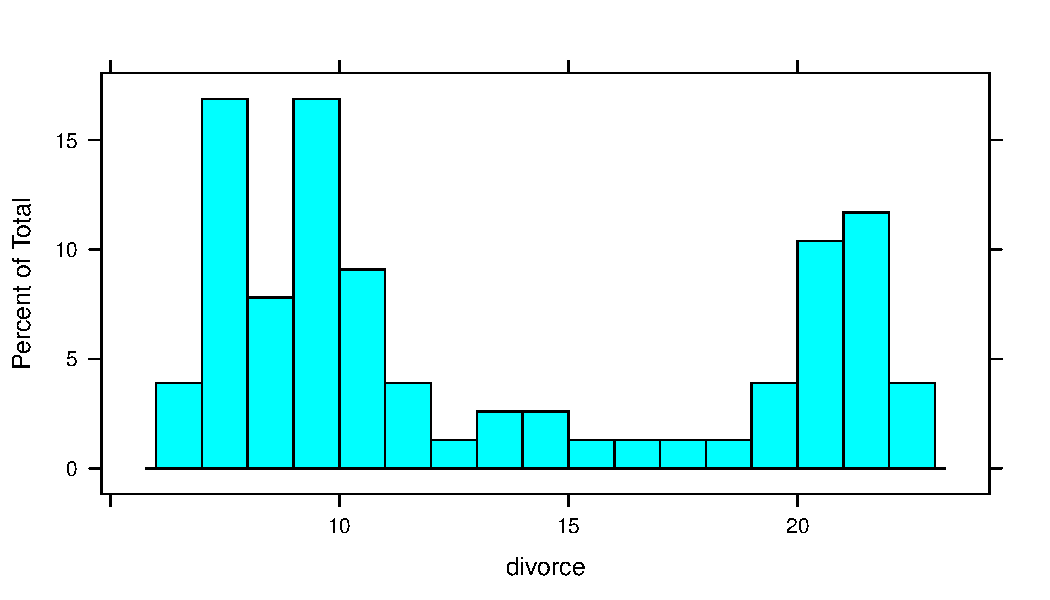
\includegraphics[width=\maxwidth]{figure/histograms-1} \caption[Histogram of the status variable]{Histogram of the status variable}\label{fig:histograms1}
\end{figure}

\begin{figure}
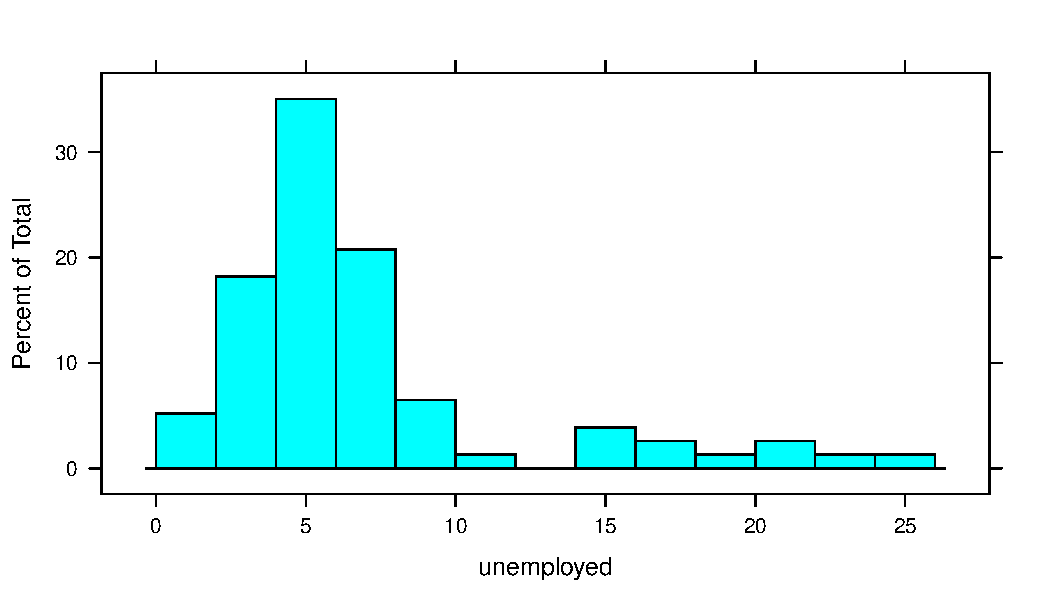
\includegraphics[width=\maxwidth]{figure/histograms-2} \caption[Histogram of the income variable]{Histogram of the income variable}\label{fig:histograms2}
\end{figure}

\begin{figure}
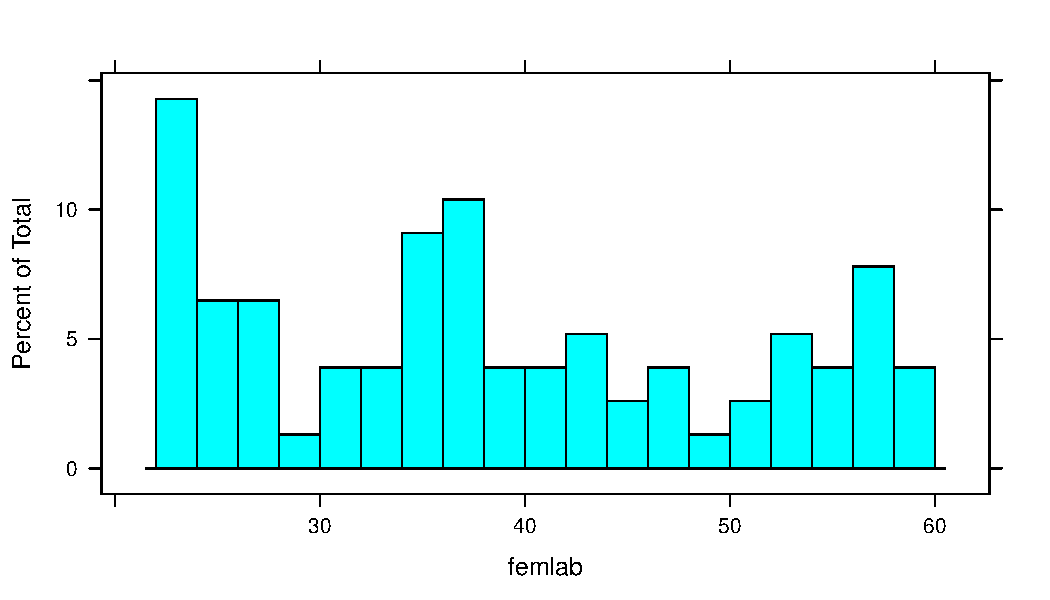
\includegraphics[width=\maxwidth]{figure/histograms-3} \caption[Histogram of the gamble variable]{Histogram of the gamble variable}\label{fig:histograms3}
\end{figure}


\end{knitrout}




\begin{knitrout}
\definecolor{shadecolor}{rgb}{0.969, 0.969, 0.969}\color{fgcolor}
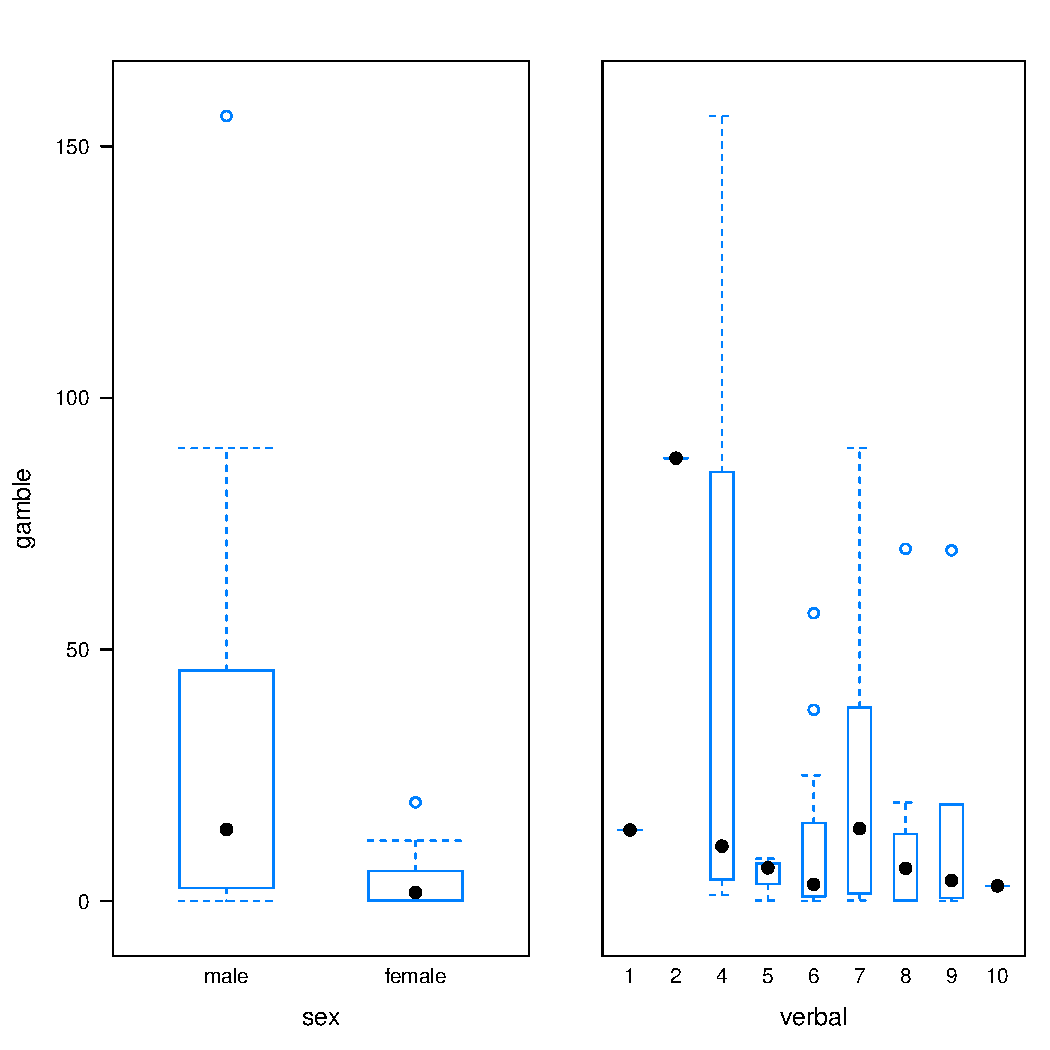
\includegraphics[width=\maxwidth]{figure/plot_objects-1} 

\end{knitrout}


\begin{knitrout}
\definecolor{shadecolor}{rgb}{0.969, 0.969, 0.969}\color{fgcolor}\begin{figure}
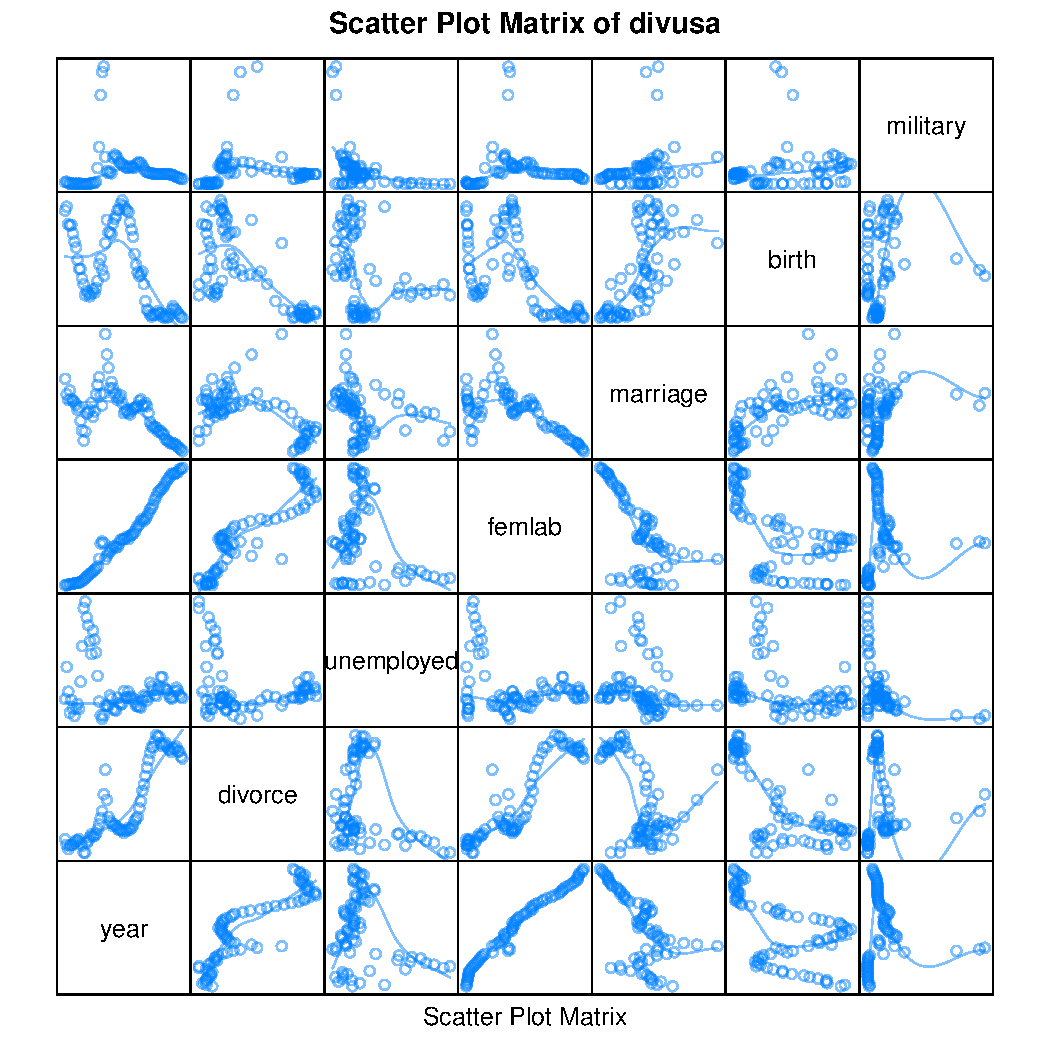
\includegraphics[width=\maxwidth]{figure/splom-1} \caption[multi-variate comparisons]{multi-variate comparisons}\label{fig:splom}
\end{figure}


\end{knitrout}


\begin{knitrout}
\definecolor{shadecolor}{rgb}{0.969, 0.969, 0.969}\color{fgcolor}\begin{figure}
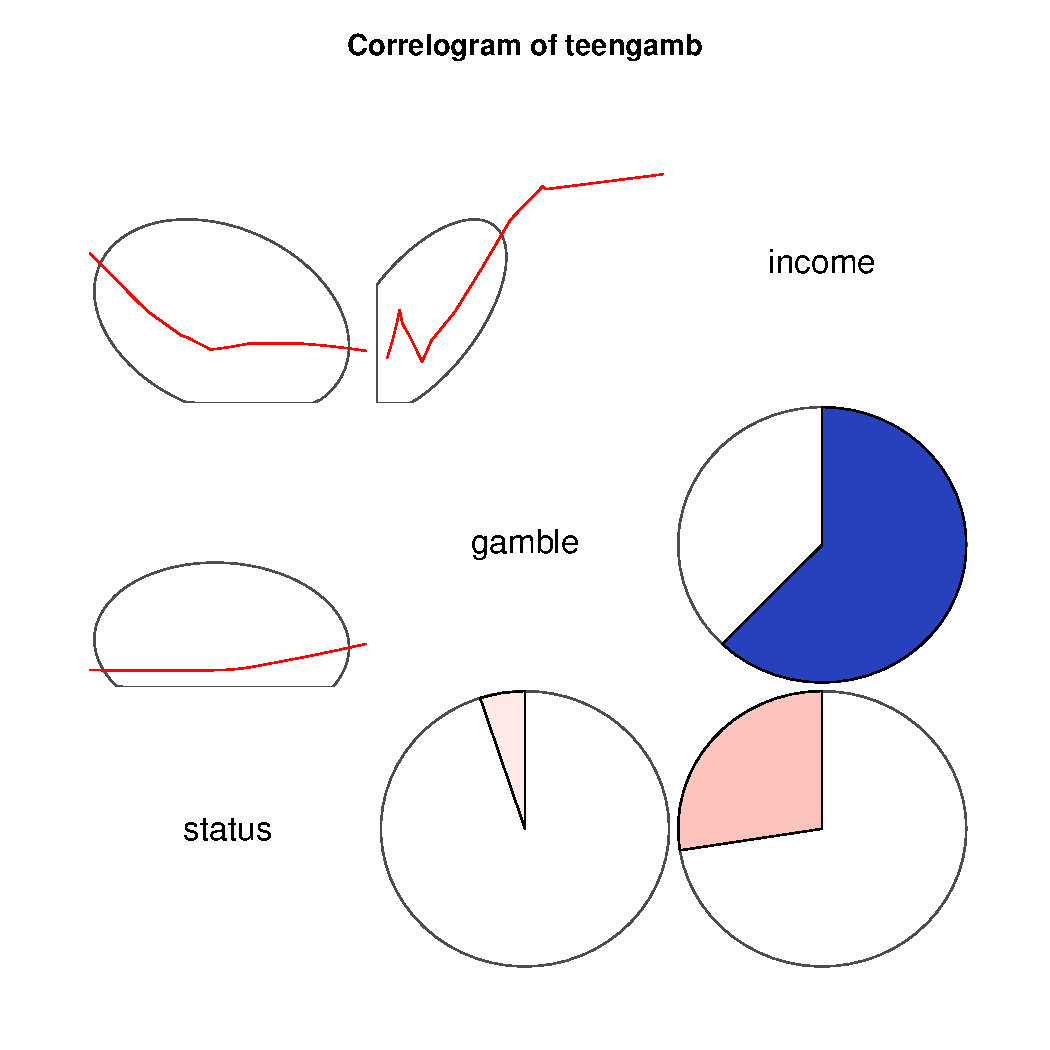
\includegraphics[width=\maxwidth]{figure/corrgram-1} \caption[multi-variate comparisons]{multi-variate comparisons}\label{fig:corrgram}
\end{figure}


\end{knitrout}


\begin{knitrout}
\definecolor{shadecolor}{rgb}{0.969, 0.969, 0.969}\color{fgcolor}\begin{kframe}
\begin{verbatim}
## 
## 	Welch Two Sample t-test
## 
## data:  gamble by sex
## t = 3.6227, df = 28.503, p-value = 0.001123
## alternative hypothesis: true difference in means is not equal to 0
## 95 percent confidence interval:
##  11.27085 40.54758
## sample estimates:
##   mean in group male mean in group female 
##            29.775000             3.865789
\end{verbatim}
\end{kframe}
\end{knitrout}

\begin{knitrout}
\definecolor{shadecolor}{rgb}{0.969, 0.969, 0.969}\color{fgcolor}\begin{kframe}
\begin{alltt}
\hlcom{# Sex has been coded as integer values 0}
\hlcom{# and 1. 40% of the observations are}
\hlcom{# female.}

\hlcom{# Parents socioeconomic status is likely}
\hlcom{# to be a percentage ranging between 18}
\hlcom{# and 75.}

\hlcom{# Verbal may be an indicator of education}
\hlcom{# with discrete levels 1 - 10 (maximum of}
\hlcom{# possible 12 indicated in the help).}

\hlcom{# There don't appear to be any missing}
\hlcom{# values. Where zeros appear, they seem}
\hlcom{# to be reasonable values.}

\hlcom{# set factors correctly}
\hlstd{df} \hlkwb{<-} \hlkwd{mutate}\hlstd{(df,} \hlkwc{sex} \hlstd{=} \hlkwd{factor}\hlstd{(sex,} \hlkwc{labels} \hlstd{=} \hlkwd{c}\hlstd{(}\hlstr{"male"}\hlstd{,}
    \hlstr{"female"}\hlstd{)),} \hlkwc{verbal} \hlstd{=} \hlkwd{factor}\hlstd{(verbal,} \hlkwc{levels} \hlstd{=} \hlnum{1}\hlopt{:}\hlnum{12}\hlstd{))}
\end{alltt}
\end{kframe}
\end{knitrout}

\end{document}
